% Chapter 1

\chapter{Graph based in-situ analytics} % Main chapter title

\label{Chapter6} % For referencing the chapter elsewhere, use \ref{Chapter1}

\lhead{Chapter 6. \emph{Graph based in-situ analytics}} % This is for the header on each page - perhaps a shortened title

%----------------------------------------------------------------------------------------
\section{The need for in-situ analytics}
Parallel simulations produce large amount of data. The traditional approach consists of writing this data to disk, reading it back from the disk and analyzing it. But this approach is extremely slow. An alternative would be to analyze the data online, as soon as it is provided by the simulation, before writing it to the disk. Thus the data is reduced in size before being written to the disk, which leads to a better performance.

%----------------------------------------------------------------------------------------
\section{The proposed algorithm}    %[TODO] where did this algorithm come from? why is this being done?
A variety of molecular (mechanical and biological) simulations, generate a large number of (from a few million to a few hundred million) points in a three dimensional space. The interactions between such molecules/points determines the position of the points generated in the next time-step of the solution. Hence the following (two dimensional) algorithm becomes a crucial step in the analytics on the data produced by these simulations:

\begin{enumerate}
\item Hash the set of points into squares in the 2D space using four different hash functions.
\item For each square in a given hash, make an undirected graph with an edge between two points \emph{iff} the euclidean distance between them is less than a given threshold {T}. This is an empirical parameter of the algorithm.
\item Fuse all graphs hence formed.
    \begin{itemize}
        \item For each point, unionize the four adjacency lists (formed in \texttt{Step 2}) corresponding to the four hash functions.
        \item Concatenate all such adjacency lists (one for each point) into a single graph.
    \end{itemize}
\item Output a set of connected components for this graph.
\end{enumerate}
The aforementioned hash functions tile the entire 2D space into several squares, each of side \begin{math}2\times{T}\end{math}. For a given point \begin{math} (x, y) \end{math}, a hash function hence outputs the co-ordinates of the square in which this point lies.

Hence, one such hash function would map \begin{math} (x, y) \end{math} to \begin{math} (\frac{x}{2\times{T}}, \frac{y}{2\times{T}}) \end{math}. The other three hash functions mentioned are obtained by shifting the origin of the 2D space to \begin{math}(0, \frac{T}{2}), (\frac{T}{2}, 0) \end{math}, and \begin{math}(\frac{T}{2}, \frac{T}{2})\end{math} respectively.

    The above design implies that for any two points that are at a distance of \begin{math} T \end{math} or less, they will be hashed into the same square in atleast one of the four hashes. Therefore there would be \begin{math} {4\times{O({(4n{\frac{T}{R}})}^2)}} \end{math} distance computations where \begin{math} R \end{math} is the range of the 2D space, instead of the naive \begin{math} {O(n^2)} \end{math}. This constant factor is quite meaningful because the threshold distance is up to 4 orders of magnitude less than the range.
[ADD A FIGURE OF HASHES]
%----------------------------------------------------------------------------------------
%\section{Code}
\section{Profiling}
This sequential algorithm was profiled using valgrind and the key areas of optimization were identified to be \texttt{Step 2} and \texttt{Step 3}.
\begin{figure}%[opt-rat]
	%\centering
    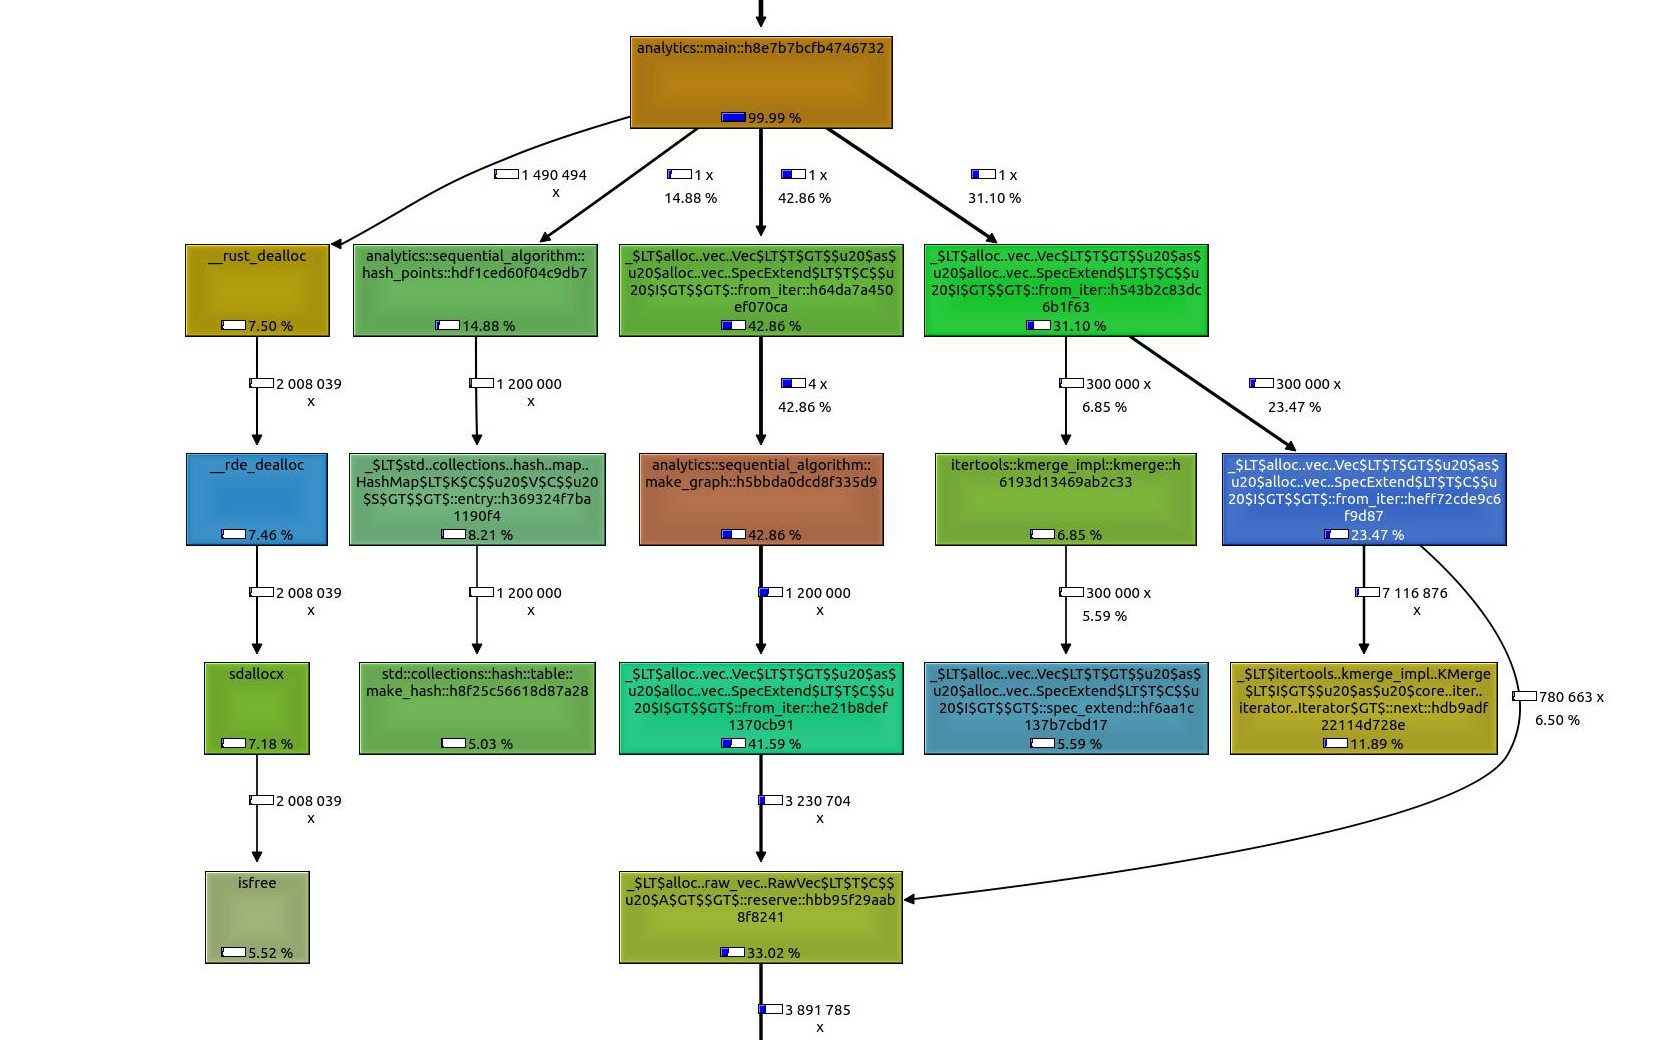
\includegraphics[scale=0.4]{Pictures/profile.png}
		\rule{40em}{0.5pt}
    \caption[Profiling]{Call graph generated by kcachegrind.}
	\label{fig:profile}
\end{figure}

\section{Some optimizations}
The following sections detail the sequential optimizations that were carried out to improve the run-time of the algorithm.
\subsection{Optimizing graph fusion}
It was evident from the profile that a function \texttt{kmerge()} was taking up more than \begin{math} 16\% \end{math} time, and hence the contribution of \texttt{Step 3} in the overall run time was unusually high. This function was being used (from an external library) to merge two sorted iterators. However, it had been written to be used for any number of sorted iterators, and hence the implementation internally used a heap to order these iterators. While this would have been a nice strategy for a significantly large number of iterators, in the case of two iterators, it led to an unnecessary overhead.

Therefore, this was replaced with a handwritten function to fuse two sorted iterators into one.

\subsection{Optimizing graph creation}
A rather complicated optimization was carried out to reduce the number of distance computations within a hash square as well (\texttt{Step 2}). The above design relied on the threshold in order to reduce the number of distance computations, however with the following geometric optimization, the correlation between the threshold and the performance was significantly reduced.

The objective of this optimization is to build a smaller set of points out of all the points in a square, following which, distance computation will be done only for the points in the smaller set. This is done in the following manner:
\begin{enumerate}
        \item Rehash the points in a square by tiling it with even smaller squares, such that no two points in the same inner square are more than \begin{math} T \end{math} distance apart. Hence the side of the inner square must be \begin{math} \frac{T}{\sqrt2} \end{math}.
            \begin{itemize}
            \item This implies that all the points in an inner square form a clique of the final graph.
            \item However, there might exist edges between two points that are not in the same clique.
            \item Hence, distance computation must still be done between all points of the first clique and all the points of the second clique for all unordered pairs of cliques that can be formed.
            \item However, if there exists a subset of \emph{relevant points} in a clique, such that for any point outside the clique, the point within the clique that is closest to it must be a part of this subset of \emph{relevant points}, then distance computation is not required for any point that is not in this subset.
            \end{itemize}
        \item The problem hence reduces to determining that for a given square with a lot of points inside it, which are the points that can never be the ones closest to a point outside this square.
        \item This can be further simplified to compute a set of \emph{relevant points} for each side of the square and then take an union of all such sets of \emph{relevant points}.
        \item Hence for any two sets of relevant points \begin{math} R1, R2 \end{math} obtained from two different inner squares (within the same outer square), distance computation is only done between %\begin{math} P1, P2\end{math} : \begin{math}\forall P1 \in R1 \end{math} and \begin{math} \forall P2 \in R2\end{math}
\end{enumerate}
The following section describes how to compute the set of relevant points.

%----------------------------------------------------------------------------------------
\subsection{Computing the relevant points}
\begin{figure}%[opt-rat]
	%\centering
        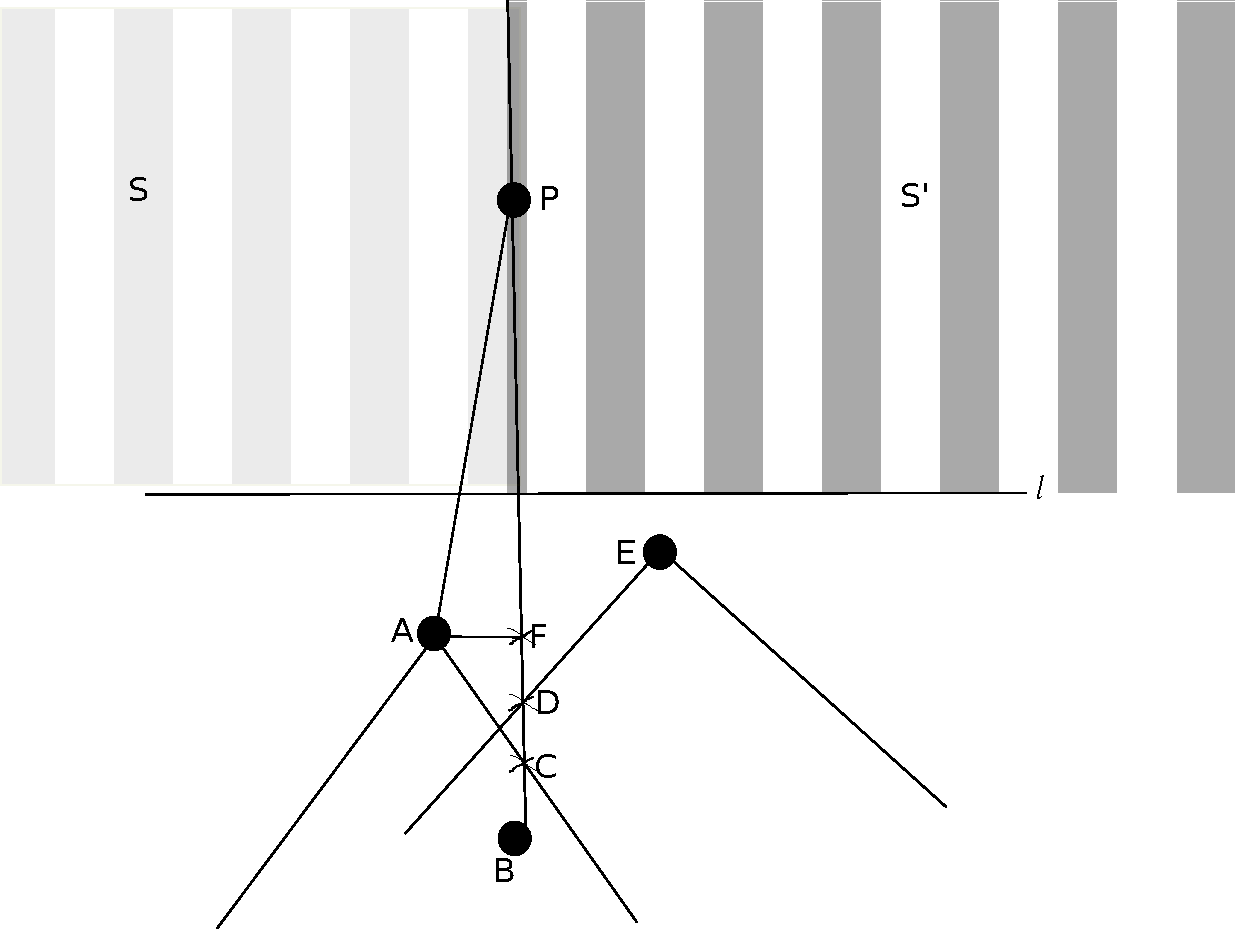
\includegraphics{Figures/optimization-rationale.pdf}
		%\rule{35em}{0.5pt}
    \caption[Optimization]{The rationale behind the optimization.}
	\label{fig:opt-rationale}
\end{figure}
The figure \ref{fig:opt-rationale} demonstrates the rationale behind the computation of the relevant points.
\begin{enumerate}
    \item For a given point $A$, draw two lines with angles 45$^\circ$ and 135$^\circ$.
    \item Conjecture: For any point $B$ below these lines, there can never exist any point in the area $S$ (on the left side of the vertical line passing through $B$) such that the distance between that point and $B$ is less than the distance between that point and $A$.
        \begin{itemize}
            \item Consider the point $P$ which is on the boundary of $S$. \begin{equation} d(P, C) = d(P, F) + d(F, C) \end{equation} and since slope of $AC$ is $-1$, \begin{equation} d(A, F) = d(F, C) \end{equation} and in triangle $APF$, \begin{equation} d(P, A) < d(F, A) + d(P, F) \end{equation} therefore \begin{equation} d(P, A) < d(P, C) < d(P, B) \end{equation}
            \item It is easy to see that this holds if we move point $P$ anywhere in the area $S$.
        \end{itemize}
    \item The same argument is made for any point in the area $S'$ using points $E$ and $D$.
    \item The conclusion in such a scenario is that point $B$ can never be in the set of \emph{relevant points} for the line $l$ given that points $A$ and $E$ are relevant.
\end{enumerate}

The algorithm to find the \emph{relevant points} hence proceeds in a similar fashion by evaluating for each side of the square, which points are relevant and then taking the union of all such points.
However, this optimization itself costs $O(n\log{n})$ where $n$ is the number of points in the smaller square. Furthermore, the number of points it ends up reducing is also completely dependent on the density of the inner square. Hence, some benchmarking was carried out to find out at approximately how many points per square should this optimization be performed.
\begin{figure}%[opt-rat]
	%\centering
    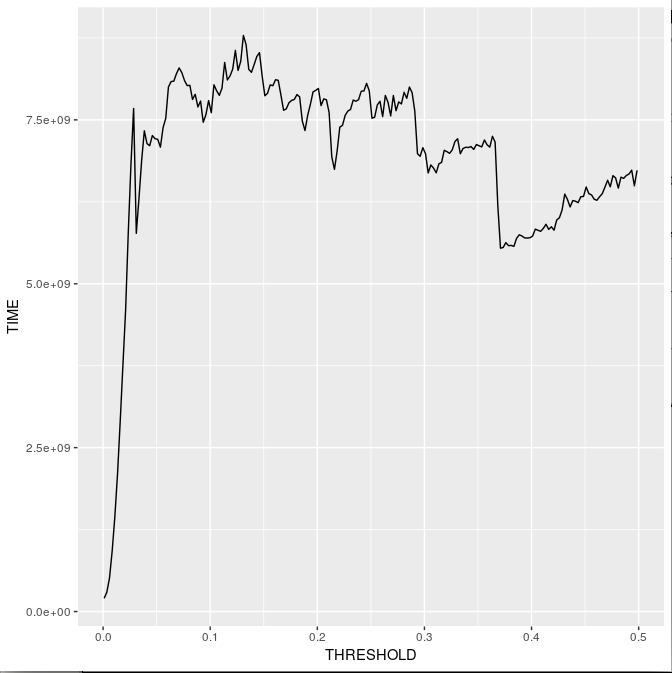
\includegraphics[scale=0.7]{Pictures/optimization_benchmark.png}
		%\rule{35em}{0.5pt}
    \caption[Optimization]{Time taken (in nanoseconds) versus Threshold (Range of the 2D space is (0,1))}
	\label{fig:opt-bench}
\end{figure}


The Figure \ref{fig:opt-bench} shows the dependence of the run-time on the threshold parameter in the final hybrid algorithm. This was programmed to switch on the optimization once the number of points crosses $500$ in any given square.
